\renewcommand{\SS}{\mathbb{S}}
\newcommand{\Par}[2]{\mbox{$( #1, #2 )$}}

\chapter{Uvod do molekularnej genetiky a bioinformatiky}

Na zaciatku prace strucne zoznamime citatela s vybranymi pojmami
z bioinformatiky i genetiky.

\section{Co je RNA}

Nositelkami genetickej informacie bunky su molekuly nukleovych kyselin
tvorene retazcami nukleotidov, ktore su zakladnymi stavebnymi jednotkami
nukleovych kyselin. Vyskytuje sa niekolko variant nukleotidov (baz). U RNA su to
adein (A), guanin (G), cytozin (C), uracyl (U),
pri DNA sa namiesto uracylu vyskytuje tymin (T).
Medzi jednotlivymi bazami existuju vazby na principe komplementarity.
Vodikove vazby existuju medzi bazami A-U a C-G u RNA a podobne A-T a C-G u DNA.
Strukturu nukleovych kyselin mozeme chapat podla stupna zjednodusenia
\begin{itemize}
	\item Primarna struktura - je urcena poradim jednotlivych nukleotidov
		do polynukleotidoveho retazca
	\item Sekundarna struktura - je dana 2D priestorovym usporiadanim molekuly
	\item Terciarna struktura - 3D priestorove usporiadanie molekuly
\end{itemize}
DNA je dvojvlaknova molekula u ktorej spojenie medzi vlaknami sa realizuje na principe
komplementarity.
Naopak, RNA je iba jednovlaknova molekula. V snahe minimalizovat energiu molekuly,
RNA komplementaritou vytvara v molekule bazove pary. Tie tvoria sekundarnu strukturu.

V praci budeme primarnou a sekundarnou strukturou mysliet prave primarnu a sekundarnu
strukturu RNA, ak nebude povedane inak.

Az donedavna sa myslelo, ze funkcia RNA je iba pri tvorbe bielkovin (mRNA), alebo
ako transporter aminokyselin (tRNA). Avsak existuje mnoho dalsich, od relativne
malych molekul tvorenych desiatkami baz, ktore pomahaju pri expresii genov
(miRNA, siRNA, tmRNA, siRNA a dalsie), az po velke, tvorene tisickami nukleotidov (rRNA).

\begin{definice}\label{def:RNA_primarna_struktura}
	Nech $\Sigma$ je abeceda $\{A, C, G, U\}$. Potom slovo $W \in \Sigma^n$ nad touto abecedou
	je sekvencia nukleotidov (baz) RNA.
\end{definice}

%TODO: obrazok prim/sek/terc struktury RNA

\section{Sekundarna struktura rRNA + konzervovanost}

Ako hlavny objekt zaujmu sme si spomedzi RNA vybrali ribozomalnu.
Je to hlavne kvoli jej velkosti a konzervovanosti.
Konzervovanostou myslime to, ze napriec celym spektrom organizmov sa sekundarna struktura
rRNA velmi nemeni. 

\begin{definice}\label{def:RNA_sekundarna_struktura}
	Nech W je sekvencia podla definicie \ref{def:RNA_primarna_struktura} dlzky n.
	Sekundarnou strukturou oznacime mnozinu $\SS$ parov \Par{i}{j} takych, ze
	pre dva pary \Par{i}{j} a \Par{k}{l} $\in \SS$ (BUNO $i \leq k$) plati jedno z nasledujucich:
	\begin{itemize}
		\item $i = k \iff j = l$
		\item $i < j < k < l$, cize par \Par{i}{j} predchadza par \Par{k}{l}
		\item $i < k < l < j$, cize par \Par{i}{j} obsahuje par \Par{k}{l}
	\end{itemize}
\end{definice}

Prva podmienka zabezpecuje, ze nukleotid je najviac v jednom bazickom pare, druha a tretia
hovoria o usporiadani parov, bud su na sebe nezavisle alebo na seba nadvazuju.
Posledna podmienka zakazuje existenciu pseudouzlov (pseudoknots).

%TODO: 2 obrazky RNA napriec fylogenetickym stromom
%TODO: pseudoknot obrazok

\begin{figure}[H]
\centering
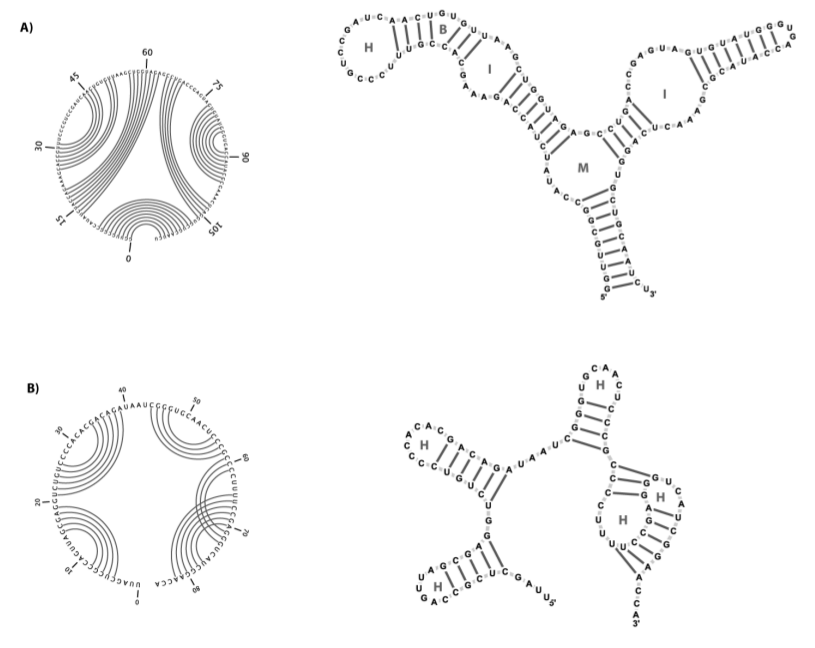
\includegraphics[width=140mm, height=120mm]{../img/RNA_circular_reprezentation.png}
\caption{Circular Feynman - kruhova reprezentacia sekundarnej struktury}
\label{obr:RNA_motifs}
\end{figure}


\subsection{Motivy}

Na obrazkoch mozeme pozorovat motivy RNA molekul, stem/loop, s dalsim
moznym delenim loopov na bulge, interior loop a multibranch loop.
V dalsom rozpravani nam bude stacit rozdelenie na stem a loop.

%TODO: ako nazyvat strukturne motivy v RNA: anglicky, alebo hladat vhodny preklad

\begin{figure}[H]
\centering
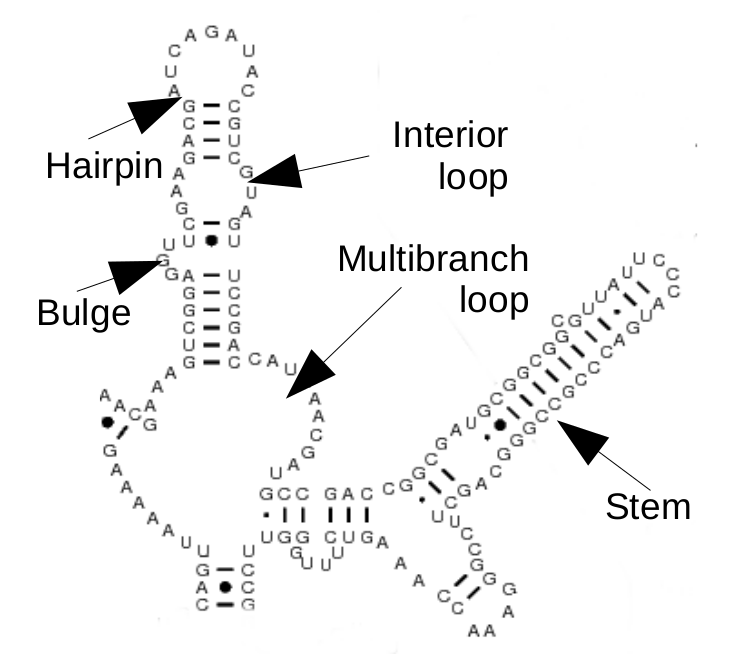
\includegraphics[width=70mm, height=70mm]{../img/struktury_v_rna.png}
\caption{Strukturalne motivy v RNA}
\label{obr:RNA_motifs}
\end{figure}

\section{Reprezentacia sekundarnej struktury}

Definicia \ref{def:RNA_sekundarna_struktura} nam ponuka reprezentovat sekundarnu strukturu
ako usporiadany les.

\begin{figure}[H]
\centering
%TODO: vlastny obrazok... namiesto clankoveho
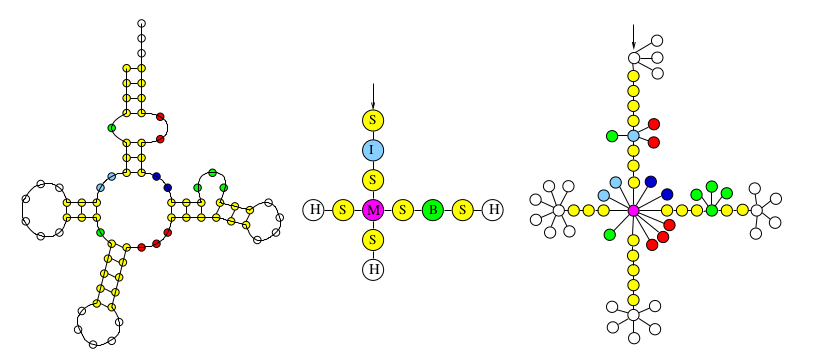
\includegraphics[width=130mm, height=70mm]{../img/stromova_reprezentacia_rna.png}
\caption{Varianty reprezentacie vrcholov}
\label{obr:RNA_vrcholy}
\end{figure}

\begin{definice}\label{def:strom}
	Usporiadany zakoreneny strom je orientovany graf, v ktorom plati, ze hrany su orientovane
	vzdy v smere z predka na potomka. Okrem korena ma kazdy vrchol svojho predka. Existuje tu
	dalej usporiadanie medzi potomkami.
	\\
	Usporiadany les je usporiadana mnozina stromov.
	%TODO: obrazok usporiadania stromov
\end{definice}

Kazdy vrchol moze reprezentovat napriklad motiv v strukture RNA, alebo nukleotid, bazovy par, ...

